\documentclass[conference]{IEEEtran}
\IEEEoverridecommandlockouts
% The preceding line is only needed to identify funding in the first footnote. If that is unneeded, please comment it out.
\usepackage{cite}
\usepackage{amsmath,amssymb,amsfonts}
\usepackage{algorithmic}
\usepackage{graphicx}
\usepackage{textcomp}
\usepackage{xcolor}
\usepackage{url}
\usepackage{float}
\usepackage{tikz}
\usepackage{booktabs}
\usepackage{subcaption}
\usepackage{lipsum} 
\usepackage{dblfloatfix}
\usepackage{bm}
\usepackage{bbm}

\def\BibTeX{{\rm B\kern-.05em{\sc i\kern-.025em b}\kern-.08em
    T\kern-.1667em\lower.7ex\hbox{E}\kern-.125emX}}
\begin{document}

\title{
    Defect Detection in Semiconductor Wafers Using Image Classification
    \thanks{Computational resources were provided by the WVU Research Computing Thorny Flat HPC cluster, partly funded by NSF OAC-1726534.}
}

% Authors 
\author{
    \IEEEauthorblockN{Ian S. Jackson}
    \IEEEauthorblockA{\textit{Lane Department of Computer Science and Electrical Engineering} \\
    \textit{West Virginia University}\\
            Morgantown, United States \\
            isj0001@mix.wvu.edu}
}

\maketitle
\thispagestyle{plain}
\pagestyle{plain}

\begin{abstract}
    Defect detection in semiconductor wafers is a critical task in high-precision manufacturing, where even minor anomalies can significantly impact device yield and reliability. 
    This study explores three pattern recognition-based image classification models—Convolutional Neural Networks (CNNs), Support Vector Machines (SVMs), and K-Nearest Neighbors (KNNs)—for multi-class wafer defect identification using the WM811K dataset. 
    The CNN model, leveraging deep hierarchical feature extraction and regularization techniques such as squeeze-and-excitation blocks and Focal Loss, achieved the highest performance with a 72.85\% test accuracy and a 0.7195 macro F1-score. 
    In contrast, the SVM model exhibited severe class bias and poor generalization, and the KNN model, while moderately accurate, was computationally inefficient for real-time deployment. 
    The results highlight the importance of model selection, class imbalance handling, and spatial feature representation in wafer defect classification. 
    Findings support CNNs as the most viable standalone solution, with future work potentially benefiting from hybrid or ensemble methods to enhance performance on rare or ambiguous defect types.
\end{abstract}

%-- Introduction --%
\section{Introduction}
Defect detection is a critical process in the semiconductor manufacturing industry. 
Traditional inspection methods often rely on manual analysis or rule-based systems, which can be time-consuming and prone to human error.
Additionally, the increasing complexity and miniaturization of semiconductor devices necessitate highly precise defect detection methods to ensure manufacturing yield and device reliability.
Semiconductor wafer defects, such as cracks, scratches, and contamination, can significantly impact the performance and lead to costly failures. 
Recent advancements in deep learning and computer vision have enabled automated defect detection using image classification models, offering improved accuracy and efficiency \cite{b1}.

In this work, I propose to explore and analyze deep learning-based and pattern recognition-based approaches for multi-class defect classification in semiconductor wafers. 
Specifically, the project will investigate convolutional neural networks (CNNs), support vector machines (SVMs), and k-nearest neighbors (KNNs) for their effectiveness in classifying defects from high-resolution wafer images. 
% CNNs, known for their outstanding performance in image recognition tasks \cite{b2}, will be a primary focus. 
% Additionally, a fusion model that integrates the strengths of these methods will be developed to further enhance classification performance.

%-- Background --%
\section{Background}
\subsection{Semiconductor Manufacturing and Defect Detection} 
Semiconductor manufacturing is a complex, multi-step process that involves the fabrication of integrated circuits (ICs) on silicon wafers. 
Silicon, due to its semiconducting properties and abundance, serves as the foundational substrate upon which microelectronic devices are constructed. 
The process begins with the production of ultrapure silicon, which is then sliced into thin wafers and subjected to a sequence of photolithographic, deposition, etching, and doping steps to create intricate circuit patterns \cite{bg1}.

Throughout the fabrication cycle, maintaining the structural and electrical integrity of the wafer is critical. 
Even microscopic defects on the wafer surface—such as particles, scratches, voids, or crystal dislocations—can lead to performance degradation or complete failure of the resulting ICs. 
As device geometries shrink and circuit densities increase, the tolerance for such defects becomes even more stringent, making defect detection and classification an essential component of the manufacturing workflow.

To ensure high yield and reliability, semiconductor foundries implement rigorous in-line and end-of-line inspection protocols using various types of imaging and metrology tools. 
These inspections generate large volumes of wafer surface data, which must be analyzed for the presence and nature of defects. 
This challenge has led to the adoption of automated pattern recognition and machine learning methods to improve accuracy and efficiency in identifying defect patterns and sources \cite{bg2}.

Historically, defect inspection involved rule-based visual algorithms and manual review, but these techniques are becoming insufficient. 
Traditional algorithms struggle with generalizing across diverse defect types and varying image conditions \cite{bg3}. 
In response, manufacturers are increasingly deploying automated, intelligent systems based on pattern recognition and machine learning to enhance defect detection accuracy and consistency. 
% Their integration aligns with broader smart manufacturing efforts under Industry 4.0, which aim to reduce human error, enable real-time decision-making, and support adaptive quality control [5].

%~~ Sample Wafer Images ~~%
\begin{figure*}[t]
    \centering
    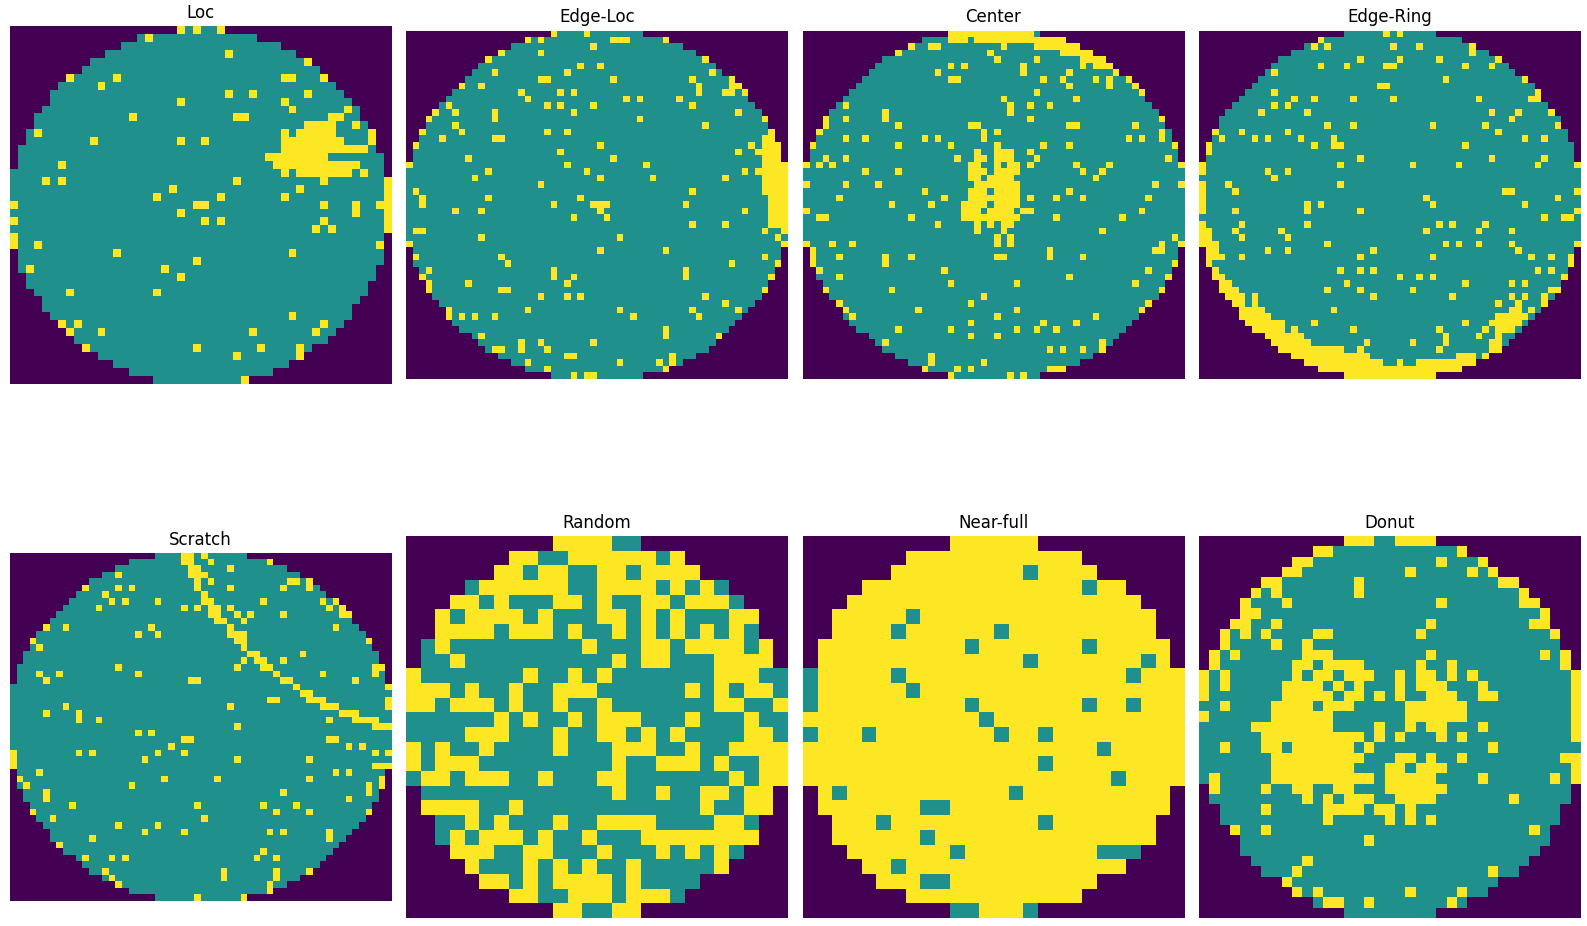
\includegraphics[width=0.9\textwidth]{assets/sample_wafer_maps.png}
    \caption{Sample wafer images from the WM811K dataset, illustrating various defect types: (a) Loc, (b) Edge-Loc, (c) Center, (d) Edge-Ring, (e) Scratch, (f) Random, (g) Near-full, and (h) Donut.}
    \label{fig:sample-wafers}
\end{figure*}

\subsection{Review of Common Techniques}
A wide range of pattern recognition techniques have been applied to automate defect detection in silicon wafer inspection, each with distinct strengths depending on the complexity and type of image data. 
Among the most widely used are Convolutional Neural Networks (CNNs), which have become the de facto standard for image-based classification tasks due to their ability to learn hierarchical feature representations. 
CNNs are especially effective at distinguishing subtle variations in defect morphology by learning spatial features directly from pixel intensities, eliminating the need for manual feature extraction \cite{bg4}. 
% In wafer inspection tasks, CNNs have achieved high classification accuracy on datasets with complex noise patterns and multiple defect classes, often outperforming traditional methods [2].

Other approaches include Support Vector Machines (SVMs), which are supervised learning models well-suited for small to medium-sized datasets. 
SVMs construct optimal decision boundaries between defect types by maximizing the margin between data points of different classes, and have proven effective when combined with image preprocessing steps such as Principal Component Analysis (PCA) or texture-based feature extraction \cite{bg5}. 
For faster models, K-Nearest Neighbors (KNN) is also employed, especially in cases with well-clustered defect types. 
Although less computationally efficient for large datasets, KNN offers simplicity and flexibility in non-linear classification scenarios \cite{bg6}. 
% Hybrid techniques that combine CNN-based feature extraction with classical classifiers like SVM or decision trees have also gained attention for balancing accuracy and interpretability [5]. 
% The continued evolution of these pattern recognition methods offers promise for more robust, scalable, and adaptive wafer inspection systems.

%-- Related Work --%
\section{Related Work} 
\subsection{Convolutional Neural Networks}
CNNs have been widely adopted for wafer defect classification due to their powerful feature extraction capabilities. 
Bao et al. \cite{rw1} proposed a method combining autoencoder-based data augmentation with CNNs to address class imbalance and noise in wafer defect maps, achieving a classification accuracy of 98.56\% on the WM-811K dataset. 
Similarly, Ang et al. \cite{rw2} conducted a comparative study of pretrained CNN models, including MobileNet-v2 and ResNet-50, finding that MobileNet-v2 outperformed others in terms of accuracy and computational efficiency. 
Jeong et al. \cite{rw3} introduced a geometric transformation-invariant CNN model that maintained high classification performance even with limited training data by incorporating rotation and flip invariance.

\subsection{Support Vector Machines}
SVMs have been effectively utilized, often in conjunction with deep learning models, for wafer defect classification. 
Behera et al. \cite{rw4} employed deep features extracted from ResNet-101 to train an SVM classifier, optimizing hyperparameters through various techniques and achieving an accuracy of 88.1\%. 
Lim et al. \cite{rw5} explored a transfer learning pipeline where features from DenseNet models were classified using linear SVMs, resulting in a test accuracy of 86\%.

%~~ CNN Model Diagram ~~%
\begin{figure*}[t]
    \centering
    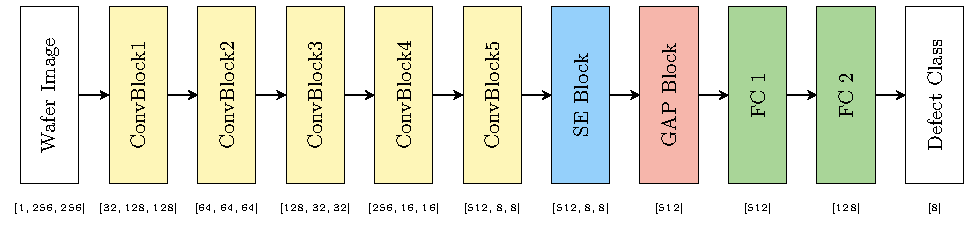
\includegraphics[width=0.9\textwidth]{assets/cnn-model.pdf}
    \caption{CNN model architecture for wafer defect classification. The model consists of multiple convolutional layers, batch normalization, max-pooling, and a squeeze-and-excitation block, followed by fully connected layers for final classification. Output dimensions given below each block, denoted by \textit{[channels, height, width]}.}
    \label{fig:cnn-model}
\end{figure*}

\subsection{Hybrid Approaches}
Combining CNNs with SVMs or KNNs has shown promise in enhancing classification performance. 
A study by Cheon et al. \cite{rw6} introduced a voting-based ensemble feature network that integrated multiple pretrained CNN models, improving defect classification accuracy on real-world wafer data. 
Additionally, a method combining CNNs with KNN classifiers was proposed for wafer surface defect classification, demonstrating improved robustness against noise and variations in defect patterns \cite{rw7}.

%-- Approach --%
\section{Approach} 
This section outlines the methodology for defect detection in semiconductor wafers using image classification techniques.
The approach consists of several key steps: dataset selection and preprocessing, training, and evaluation.

%- Dataset Description -%
\subsection{Dataset Description}
The WM811K dataset is a publicly available collection of 811,457 wafer map images released by Taiwan Semiconductor Manufacturing Company (TSMC) \cite{b2}. 
Each wafer map represents the spatial distribution of manufacturing test results on a semiconductor wafer, where pixels indicate the pass/fail status of test sites. 
The maps are primarily used for failure pattern recognition and are formatted as binary or grayscale images. 
The dataset includes a mix of labeled failure patterns and defect-free samples, providing a comprehensive base for training, validation, and testing of machine learning models.
Each sample is annotated with one of nine labels corresponding to known failure types: Center, Donut, Edge-Loc, Edge-Ring, Loc, Near-full, Random, Scratch, or None (indicating no defect). 
A sample of the wafer images can be seen in Figure \ref{fig:sample-wafers}, which illustrates various defect types present in the dataset.

Preprocessing steps include normalization of pixel values, padding to ensure consistent image dimensions, and augmentation techniques. 
This involves horizontal and vertical flipping, rotation, and scaling to increase the dataset's diversity and robustness.

% %- Training -%
% \subsection{Training}

%- Evaluation -%
\subsection{Evaluation}
To assess model performance on wafer failure pattern classification, we use three key evaluation metrics: accuracy, F1-score, and inference time. 
Each metric provides different insights into the model's effectiveness and suitability for deployment in a semiconductor manufacturing environment.

Accuracy is a basic performance metric that measures the proportion of correctly classified samples over the total number of samples. 
It is defined as:
\begin{equation}
    \text{Accuracy} = \frac{\text{TP} + \text{TN}}{\text{TP} + \text{TN} + \text{FP} + \text{FN}}
\end{equation}

The F1-score is a more robust metric that balances precision and recall, particularly useful when dealing with class imbalance. 
It is the harmonic mean of precision and recall:
\begin{equation}
    \text{F1} = 2 \cdot \frac{\text{Precision} \cdot \text{Recall}}{\text{Precision} + \text{Recall}}
\end{equation}
Where precision is the ratio of true positive predictions to the total predicted positives, and recall is the ratio of true positive predictions to the total actual positives.
We compute the macro-averaged F1-score across all classes to treat each defect type equally, regardless of frequency. 
This ensures that rare but critical defect patterns, like "Donut" or "Scratch," are evaluated fairly and not overshadowed by dominant classes.

Inference time measures how long the model takes to classify a single wafer map during deployment. 
It is expressed in seconds (s) per sample and is critical for real-time manufacturing applications. 
A high-performing model with long inference time may be impractical in fast-paced environments where throughput is essential. 
Therefore, we report average inference time per sample to evaluate deployment feasibility.

%-- Model Description --%
\section{Model Descriptions}
To differentiate between the various models used in this project, a simple naming convention is adopted.
\textit{A-class model} refers to CNN based architectures, \textit{B-class model} refers to SVM based architectures, and \textit{C-class model} refers to KNN based architectures.
Each of these models have a number of variations, which are denoted by a number after the class name.

%- A-class Model: CNN -%
\subsection{A-class Model: CNN}
The presented CNN model is a deep hierarchical feature extractor designed for multi-class image classification, outputting class probabilities for 8 distinct categories. 
The architecture follows a standard convolution-batchnorm-ReLU-pooling design pattern and is further enhanced with modern regularization techniques such as Dropout and Squeeze-and-Excitation (SE) blocks. 
The model balances complexity and generalization capacity to capture both local and global patterns within high-resolution images.

\begin{figure}[h]
    \centering
    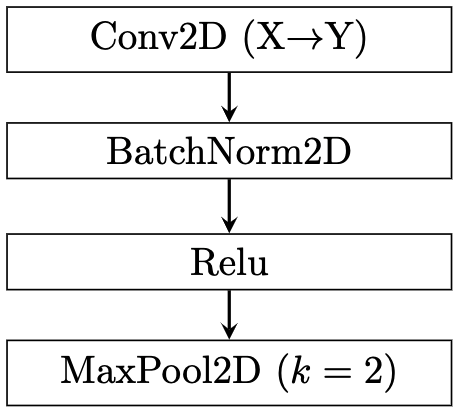
\includegraphics[width=0.45\linewidth]{assets/ConvBlock.png}
    \caption{ConvBlock architecture used in the CNN model.}
    \label{fig:conv-block}
\end{figure}

The model begins with a 2D convolutional layer using a 3x3 kernel and a stride of 1, which applies learnable filters over the input image.
The allows the model to extract low-level features such as edges, corners, and textures. 
The input image is grayscale, resulting in a single channel, and the first convolutional layer outputs 32 feature maps.
Each convolutional layer is mathematically a discrete convolution operation, defined as:
\begin{equation}
    Y_{i,j,k} = \sum_{c=1}^{C_{in}} \sum_{m=-1}^{1} \sum_{n=-1}^{1} X_{i+m,j+n,c} \cdot W_{m,n,c,k}
\end{equation}
where \(Y\) is the output feature map, \(X\) is the input image, \(W\) is the filter kernel, and \(C_{in}\) is the number of input channels.

This structure is stacked through five convolutional layers with increasing filter sizes (32, 64, 128, 256, and 512) and decreasing spatial dimensions through max-pooling layers.
Early layers learn local features, while deeper layers capture more abstract and high-level representations.

After each convolutional block, a Batch Normalization (BN) layer is applied to normalize the output of the previous layer.
This normalizes the activations across the mini-batch to zero mean and unit variance.
This helps stabilize and accelerate training by reducing internal covariance shift.

Then a max-pooling layer is applied to downsample the feature maps, reducing spatial dimensions while retaining important features.
The pooling operation is defined as:
\begin{equation}
    Y_{i,j,k} = \max_{(m,n)\in [0,1]^2} X_{2i+m,2j+n,k}
\end{equation}
This reduces the computational load and helps the model become invariant to small translations in the input image.
The 2D convolution, batch normalization, and max-pooling layers are defined as a \textit{ConvBlock} in the model.
A single ConvBlock is illustrated in Figure \ref{fig:conv-block}.

After five convolutional blocks, a Squeeze and Excitation (SE) block is applied to recalibrate the feature maps.
This is done though a two-step process: squeeze and excitation.
The squeeze step computes the global average pooling of the feature maps, resulting in a channel descriptor vector.
The excitation step applies two fully connected layers with a ReLU activation function to learn the importance of each channel.
\begin{equation}
    s_c = \sigma(W_2 \cdot \text{ReLU}(W_1 \cdot z_c))
\end{equation}
where 
\begin{equation*}
    z_c = \frac{1}{H \cdot W} \sum_{i=1}^{H} \sum_{j=1}^{W} X_{i,j,c}
\end{equation*}
and \(s_c\) is used to scale the feature maps.
This allows the network to emphasize important features and suppress less relevant ones, improving the model's ability to focus on critical patterns.

The output of the SE block is then passed through a global average pooling layer, which computes the average of each feature map, resulting in a 1D vector.
This reduces the spatial dimensions to a single value per feature map, effectively summarizing the learned features.
The output is then flattened and passed through two fully connected layers with ReLU activation and a dropout layer to prevent overfitting.
The final output layer uses a softmax activation function to produce class probabilities for the 8 defect categories.
\begin{equation}
    \hat{y}_i = \frac{e^{z_i}}{\sum_{j=1}^{8} e^{z_j}}
\end{equation}
The full CNN model architecture is illustrated in Figure \ref{fig:cnn-model}.
A table summarizing the architecture of the CNN model is provided in Appendix \ref{app:cnn-architecture}.

The model is trained using Focal Loss, which is particularly effective for imbalanced datasets.
Focal Loss is defined as:
\begin{equation}
    \mathcal{L}_{FL}(p_t) = -\alpha_t (1 - p_t)^\gamma \log(p_t)
\end{equation}
where \(p_t\) is the predicted probability of the true class, \(\alpha_t\) is a balancing factor for class imbalance, and \(\gamma\) is a focusing parameter that adjusts the rate at which easy examples are down-weighted.
The model utilizes the Adam optimizer for training. 
A summary of the training parameters is provided in Table \ref{tab:cnn_training_config} in Appendix \ref{app:cnn-architecture}.

%- B-class Model: SVM -%
\subsection{B-class Model: SVM}
The presented SVM-inspired model is a Radial Basis Function (RBF) kernel network designed to approximate the behavior of a SVM in a neural architecture. 
Unlike a traditional SVM which solves a quadratic programming problem, this model.
The flattened image is transformed into a 500-dimensional RBF feature space using a Gaussian kernel:
\begin{equation}
    \phi_j(\bm{x}) = \exp\left( -\gamma || \bm{x} - \bm{c}_j ||^2 \right)
\end{equation}
where \(\bm{c}_j\) is the center of the \(j^{th}\) Gaussian basis function, \(\gamma\) is a hyperparameter that controls the width of the Gaussian, and \(\bm{x}\) is the input image vector.
This transformation maps the input data into a non-linear feature space, allowing the model to learn complex decision boundaries.
Mathematically, this mimics the kernel trick used in traditional SVMs to construct high-dimensional feature spaces without explicitly computing the dot products:
\begin{equation*}
    K(\bm{x}, \bm{y}) = \exp\left( -\gamma || \bm{x} - \bm{y} ||^2 \right)
\end{equation*}

%~~ SVM Model Diagram ~~%
\begin{figure}[b!]
    \centering
    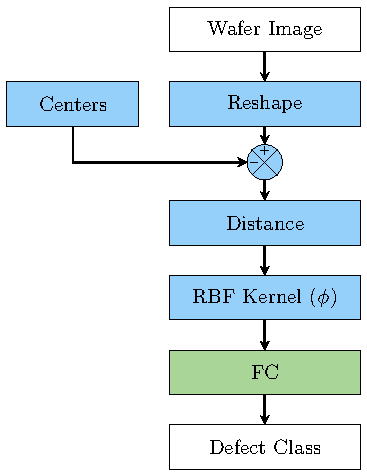
\includegraphics[width=0.7\linewidth]{assets/svm-model.pdf}
    \caption{SVM model architecture for wafer defect classification. The model consists of a radial basis function (RBF) kernel transformation followed by a fully connected layer for class probabilities.}
    \label{fig:svm-model}
\end{figure}

After RBF transformation, the model applies a fully connected (dense) layer that maps the feature space to class probabilities.
\begin{equation}
    \hat{y}_i = f_k(\bm{x}) = \bm{w}^\top_k \phi_j(\bm{x}) + b_k
\end{equation}
There is no softmax activation function in the output layer, as the model is trained using a multi-class SVM loss function.
A block diagram of the SVM model is shown in Figure \ref{fig:svm-model}.

The model uses hinge loss, extending the binary SVM theory to the multi-class case:
\begin{equation}
    \mathcal{L}_{HL} = \sum_{k\neq y} \max(0, 1 + f_k(\bm{x}) - f_{y}(\bm{x}))
\end{equation}
where \(y\) is the true class label, \(f_k(\bm{x})\) is the output of the model for class \(k\), and \(f_{y}(\bm{x})\) is the output for the true class.
This loss encourages the correct class to have a higher score than the incorrect classes by a margin of at least 1.
Unlike cross-entropy, it focuses on margin maximization rather than probability estimation, making it suitable for SVM-like architectures.
A summary of the training parameters is provided in Table \ref{tab:svm_training_config} in Appendix \ref{app:svm-architecture}.

%~~ KNN Model Diagram ~~%
\begin{figure}[t]
    \centering
    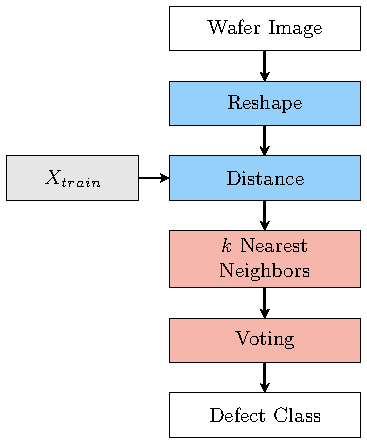
\includegraphics[width=0.7\linewidth]{assets/knn-model.pdf}
    \caption{KNN model architecture for wafer defect classification. The model flattens the input image into a 1D vector and computes distances to training samples to classify defects based on nearest neighbors.}
    \label{fig:knn-model}
\end{figure}

%- C-class Model: KNN -%
\subsection{C-class Model: KNN}
The KNN model presented here is a non-parametric, instance-based classifier applied to grayscale wafer images. 
Rather than learning weights via backpropagation, KNN memorizes the training data and makes predictions based on proximity in the feature space. 
This aligns with classical pattern recognition theory, where classification is achieved by analyzing similarity to known examples.

The model flattens the input image into a 1D vector (of size $d=65536$), similar to the SVM model.
This flattening transforms the image into a vector suitable for distance-based comparisons. 
While this discards spatial locality, it retains all pixel-level information.

The classifier stores: train features \( X_{train}\in \mathbb{R}^{N\times d} \) where $N$ is the number of training samples, 
and train labels \( y_{train}\in \{0, 1, \cdots, 7 \}^{N} \) where each label corresponds to a defect type.
The KNN model is a lazy learner, meaning it does not explicitly learn a model during training.
Instead, it stores the training data and computes distances to neighbors during inference.

For inference, the model computes the Euclidean distance between the test sample \( \bm{x} \) and all training samples \( \bm{x}_i \in X_{train} \):
\begin{equation}
    \ell(\bm{x}, \bm{x}_i) = \sqrt{\sum_{j=1}^{d} (x_j - x_{i,j})^2}
\end{equation}
This yields a distance vector \( \ell(\bm{x}, X_{train}) \in \mathbb{R}^{N} \) containing distances to all training samples.

The model then selects the \(k\) nearest neighbors based on the smallest distances, here \(k=2\).
To enhance robustness, the model uses inverse-distance weighting to assign higher weights to closer neighbors:
\begin{equation}
    s_c = \sum_{i\in \mathcal{N}_k(\bm{x})} \frac{\mathbbm{1}_{[y_i=c]}}{\ell(\bm{x}, \bm{x}_i) + \epsilon}
\end{equation}
where \( s_c \) represents the score for class \(c\), \(\mathcal{N}_k(\bm{x})\) is the set of \(k\) nearest neighbors, 
$\mathbbm{1}_{[y_i=c]}$ is an indicator function that equals 1 if the label of neighbor \(i\) is \(c\) and 0 otherwise,
and \(\epsilon\) is a small constant to avoid division by zero.
The predicted class is determined by the maximum score:
\begin{equation}
    \hat{y} = \arg\max_{c} s_c
\end{equation}
The KNN model block diagram is shown in Figure \ref{fig:knn-model}.

%-- Results --%
\section{Results} 
Each model was trained and evaluated on the WM811K dataset, with a focus on accuracy, F1-score, and inference time.
Training was performed on WVU's Thorny Flat HPC cluster, utilizing NVIDIA A100 GPUs for efficient computation.

The CNN model achieved a test accuracy of 72.85\% and an F1-score of 0.7195. The average inference time per sample was 0.0065 seconds, indicating the model's suitability for real-time or near-real-time applications.
The confusion matrix for the CNN model is shown in Figure \ref{fig:cnn_confusion_matrix}, illustrating the distribution of true and predicted labels across the 8 defect classes.
The model demonstrated strong performance in classifying common defect types such as "Edge-Loc" and "Near-full," while struggling with less frequent classes like "Donut" and "Loc."
The confusion among similar spatial defect classes (e.g., Loc, Edge-Loc, and Center) suggests that the CNN might benefit from architectural enhancements or the integration of spatial attention mechanisms to improve localization-specific classification. 
Additionally, classes with lower instance counts (e.g., Donut and Near-full) might benefit from data augmentation or class balancing techniques.

\begin{figure}[h]
    \centering
    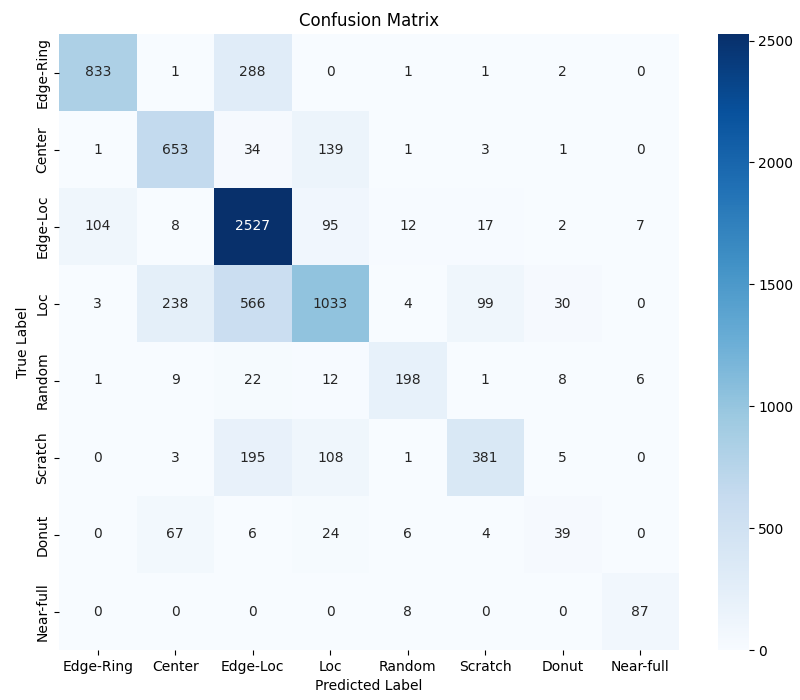
\includegraphics[width=0.9\linewidth]{assets/cnn_conf_matrix.png}
    \caption{Confusion matrix for the CNN model, showing the distribution of true and predicted labels across the 8 defect classes.}
    \label{fig:cnn_confusion_matrix}
\end{figure}

Overall, the CNN exhibits strong performance for high-frequency, spatially distinct defects, while showing room for improvement on ambiguous or visually similar classes.

The SVM model achieved a training accuracy of 56.73\% and a significantly lower test accuracy of 15.16\%, with a corresponding F1-score of 0.0764. 
Despite its extremely fast average inference time of 0.0003 seconds, the model's classification performance was insufficient for practical use.

\begin{figure}[h]
    \centering
    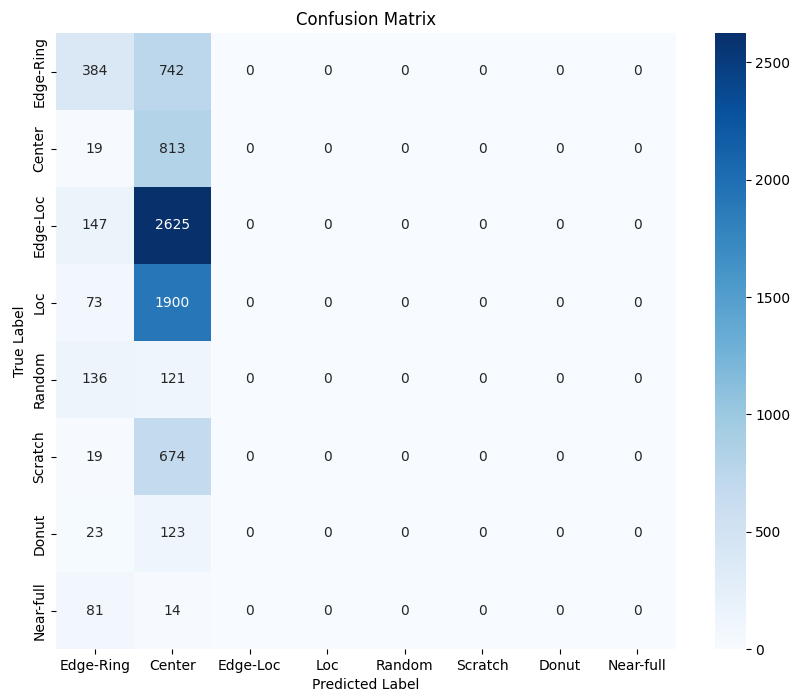
\includegraphics[width=0.9\linewidth]{assets/svm_conf_matrix.png}
    \caption{Confusion matrix for the SVM model, showing the distribution of true and predicted labels across the 8 defect classes.}
    \label{fig:svm_confusion_matrix}
\end{figure}

The confusion matrix (Figure \ref{fig:svm_confusion_matrix}) reveals severe misclassification across all defect categories. 
Notably, the SVM model consistently predicted only two classes—Edge-Ring and Center—regardless of the true class.
Nearly all samples from the Edge-Loc, Loc, Scratch, and Donut classes were incorrectly predicted as Center, with no predictions made for their correct classes.

This overwhelming class bias indicates that the SVM failed to learn meaningful decision boundaries for the multi-class problem. 
Such behavior may be attributed to the complex feature space of the dataset, high inter-class similarity, or the model's sensitivity to class imbalance. 
Additionally, the one-vs-one SVM formulation used here may not scale effectively in the presence of significant intra-class variation.
While the SVM was computationally efficient, its poor classification performance suggests it is not a viable model for this application without significant feature engineering, preprocessing, or reformulation.

\begin{figure}[h]
    \centering
    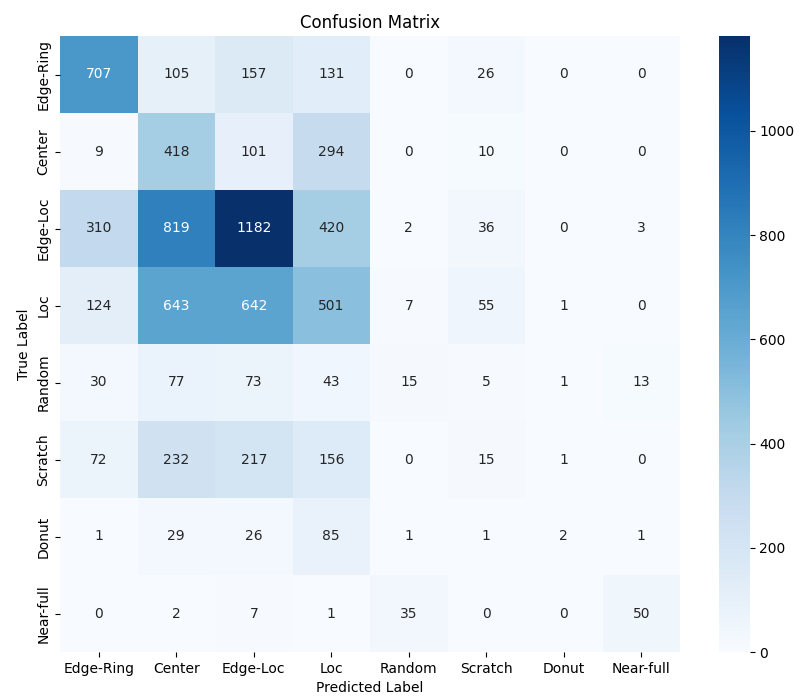
\includegraphics[width=0.9\linewidth]{assets/knn_conf_matrix.png}
    \caption{Confusion matrix for the KNN model, showing the distribution of true and predicted labels across the 8 defect classes.}
    \label{fig:knn_confusion_matrix}
\end{figure}

The KNN model achieved a test accuracy of 36.61\% and an F1-score of 0.3567, significantly lower than that of the CNN model. 
The average inference time was 2.362 seconds per sample, which is comparatively slow for real-time applications, highlighting the inefficiency of KNN on large datasets without optimization or approximation strategies.

As shown in the confusion matrix (Figure \ref{fig:knn_confusion_matrix}), the KNN model displays high confusion among spatially similar classes.
The model often confused Edge-Loc and Loc, with 1182 and 642 correctly predicted respectively, but also substantial misclassifications between the two (Edge-Loc predicted as Loc: 420; Loc predicted as Edge-Loc: 642).
Classes with fewer samples such as Donut and Near-full were underrepresented and poorly predicted (e.g., only 50 correct Near-full predictions out of 95).
Misclassification was particularly problematic between the four dominant spatial defect types—Edge-Ring, Center, Edge-Loc, and Loc—suggesting that KNN's distance-based decision boundaries were insufficient for distinguishing subtle spatial variations in feature distributions.

While KNN did retain some predictive power across all classes and had no complete blind spots, its poor scalability and long inference time make it unsuitable for deployment in its current form. 
Performance could potentially be improved by dimensionality reduction (e.g., PCA), optimized indexing (e.g., KD-Trees or Ball Trees), or switching to approximate KNN methods.

\begin{table}[h!]
    \centering
    \caption{Model Performance Summary for Wafer Defect Classification}
    \begin{tabular}{lcccc}
    \toprule
    \textbf{Model} & \textbf{Train Acc.} & \textbf{Test Acc.} & \textbf{F1-Score} & \textbf{Avg. Inf. (s)} \\
    \midrule
    CNN  & \textbf{74.31\%} & \textbf{72.85\%} & \textbf{0.7195} & 0.0065 \\
    SVM  & 56.73\% & 15.16\% & 0.0764 & \textbf{0.0003} \\
    KNN  & --       & 36.61\% & 0.3567 & 2.3620 \\
    \bottomrule
    \end{tabular}
    \label{tab:model_performance}
\end{table}

Table \ref{tab:model_performance} summarizes the performance of three models on the wafer defect classification task. 
The CNN outperforms the others across all major metrics: training accuracy, test accuracy, and F1-score, while the SVM, despite having the fastest inference time, performs poorly in both accuracy and precision. 
The KNN model shows moderate classification performance but suffers from a significantly higher inference time.

%-- Discussion --%
\section{Discussion}
This study investigated three distinct models (CNN, SVM, and KNN) for the classification of semiconductor wafer defects using the WM811K dataset. 
These models represent core methodologies in pattern recognition theory: feature-learning models (CNNs), kernel-based classifiers (SVMs), and instance-based classifiers (KNNs). 
The results clearly highlight how the intrinsic nature of the wafer defect patterns, coupled with the model's representational and decision-making capabilities, affects classification performance.

\subsection{Pattern Recognition Intuition and Model Behavior}
Pattern recognition theory tells that effective classification requires models to extract discriminative features that separate classes in the input space. 
CNNs embody this principle by hierarchically learning spatial features through convolutional layers. 
This feature abstraction explains their superior performance (test accuracy: 72.85\%, F1-score: 0.7195), especially for spatially distinct and frequent defect types such as Edge-Loc and Near-full. 
The model's ability to learn local edges, texture patterns, and higher-order visual structures allows it to distinguish between structured defects even when inter-class similarities are high.

However, CNN misclassifications in classes like Loc, Center, and Donut suggest that certain spatial patterns overlap significantly or exhibit high intra-class variance. 
These findings reinforce a fundamental principle in pattern recognition: when within-class variability rivals between-class variability, even deep models may fail without spatial attention mechanisms or architectural innovations to focus on localized defect regions.

\subsection{Limitations of Traditional Pattern Recognition Approaches}
The SVM model achieved very poor generalization (test accuracy: 15.16\%, F1-score: 0.0764), highlighting a mismatch between the RBF-kernel feature space and the high-dimensional, highly variable nature of wafer maps. 
From a pattern recognition standpoint, SVMs are effective when the data is linearly separable (in transformed space) and class boundaries are crisp. 
However, wafer defect maps often involve overlapping, fuzzy class boundaries, and subtle geometric distortions. 
The SVM's reliance on fixed basis functions and margin maximization becomes a liability in such settings—especially with imbalanced class frequencies and inter-class visual similarity. 
The model's bias toward classes like Center and Edge-Ring suggests it defaulted to global trends in the data, failing to adapt to class-specific nuances.

The KNN model achieved moderate classification results (accuracy: 36.61\%, F1-score: 0.3567), with reasonable performance on common classes but poor discrimination among visually similar classes. 
KNN exemplifies classical instance-based pattern recognition, relying on proximity in feature space to make predictions. 
While theoretically optimal in infinite data regimes with well-separated classes, in practice, KNN suffers from the “curse of dimensionality” and computational inefficiency. 
Flattening images for distance computation discards spatial structure, leading to ambiguities in classes like Edge-Loc vs. Loc or Center. 
The long inference time (2.362 s/sample) further underscores the impracticality of this approach in real-world settings, especially without dimensionality reduction or approximate search algorithms.

\subsection{Role of Data Characteristics and Class Imbalance}
The performance of all models was affected by the skewed class distribution in the WM811K dataset. 
Pattern recognition literature emphasizes that imbalanced datasets lead to biased decision boundaries, particularly for models sensitive to training data density. 
This was evident in the underperformance of all three models on rare classes like Donut and Scratch. 
While the CNN partially mitigated this using Focal Loss, its confusion matrix shows the residual challenge. 
Data augmentation strategies could further improve performance by enhancing minority class representation in the feature space.

\subsection{Toward Fusion and Ensemble Approaches}
Although the CNN was the most effective single model, the study underscores the complementary strengths of different classifiers. 
Pattern recognition theory supports the idea that combining diverse hypotheses (as in ensemble learning) can reduce generalization error. 
The fusion of CNN-extracted features with simpler classifiers like SVM or KNN, especially with feature selection or metric learning, could enhance robustness against rare classes and noisy patterns. 
Prior work cited in this report supports this notion, where hybrid or ensemble models improved accuracy by leveraging both learned and memorized representations.

%-- Conclusion --%
\section{Conclusion}
This study benchmarked three distinct pattern recognition models—CNN, SVM, and KNN—for the task of multi-class defect detection in semiconductor wafers. 
Among them, the CNN model achieved the strongest performance, accurately classifying spatially distinct wafer defects with a test accuracy of 72.85\% and an F1-score of 0.7195. 
Its deep architecture, enhanced with squeeze-and-excitation blocks and Focal Loss, proved effective in learning localized and abstract features across the WM811K dataset.

The SVM and KNN models, though rooted in foundational pattern recognition theory, struggled with generalization. 
SVM exhibited severe class bias and failed to capture non-linear defect boundaries, while KNN was limited by high-dimensional input flattening and slow inference times. 
However, both models displayed isolated strengths—SVM in efficiency, and KNN in class coverage—that suggest they could be viable with further refinement.

Several paths for future research are evident. 
\textit{Improving SVM and KNN Performance}: More effort can be directed toward optimizing the SVM and KNN models. 
For SVM, this includes better kernel design, feature engineering (e.g., PCA or wavelet transformations), and class rebalancing. 
For KNN, dimensionality reduction and approximate nearest neighbor techniques may improve both accuracy and speed.

\textit{Developing Fusion Models}: A fusion approach that combines CNN-learned features with SVM or KNN classifiers could leverage the representational strength of CNNs and the decision boundary flexibility of traditional methods. 
This hybrid model may be particularly beneficial for rare or ambiguous classes that CNNs alone struggle with.

\textit{Low-Resource Deployment}: Finally, testing and optimizing these models on lower-compute devices (e.g., Raspberry Pi, Jetson Nano) could enable cost-effective, on-device defect detection in manufacturing environments that cannot support high-end GPU infrastructure.

By addressing these areas, future iterations of this work can bridge the gap between high-performance classification and practical, low-cost deployment—ensuring broader applicability across semiconductor production lines.

\begin{thebibliography}{00}
\bibitem{b1} Y. LeCun, Y. Bengio, and G. Hinton, “Deep learning,” Nature, vol. 521, no. 7553, pp. 436–444, 2015.
\bibitem{bg1} M. Shur, “Physics and Properties of Semiconductors—A Review,” in Physics of Semiconductor Devices, Hoboken, NJ, USA: John Wiley \& Sons, Ltd, 2006, pp. 5–75. doi: 10.1002/9780470068328.ch1.
\bibitem{bg2} W. Gan, “Semiconductor Wafer Defect Detection Based on Machine Learning,” Trans. Comput. Sci. Intell. Syst. Res., vol. 6, pp. 128–133, Oct. 2024. doi: 10.62051/wr098130.
\bibitem{bg3} Geng, H., Sun, Q., Chen, T., Xu, Q., Ho, T.-Y., Yu, B.: Mixed-type wafer failure pattern recognition. In: Proceedings of the 28th Asia and South Pacific Design Automation Conference, pp. 727–732 (2023)
\bibitem{bg4} LeCun, Y., Bengio, Y. \& Hinton, G. Deep learning. Nature 521, 436–444 (2015). https://doi.org/10.1038/nature14539
\bibitem{bg5} S. L. Phung, A. Bouzerdoum and D. Chai, "Skin segmentation using color and edge information," Seventh International Symposium on Signal Processing and Its Applications, 2003. Proceedings., Paris, France, 2003, pp. 525-528 vol.1, doi: 10.1109/ISSPA.2003.1224755.
\bibitem{bg6} N. Altman, "An introduction to kernel and nearest-neighbor nonparametric regression," The American Statistician, vol. 46, no. 3, pp. 175–185, 1992.
\bibitem{rw1} Y.-Y. Bao, E.-C. Li, H.-Q. Yang, and B.-B. Jia, "Wafer map defect classification using autoencoder-based data augmentation and convolutional neural network," arXiv preprint arXiv:2411.11029, 2024. [Online]. Available: https://arxiv.org/abs/2411.11029
\bibitem{rw2} K. Ang, K. M. Ang, C. K. Ang, K. Chong, S. Tiang, W. H. Lim, A. Sharma, and T. H. Lim, "Deep learning-based silicon wafer defect classification: A performance comparison of pretrained networks," in Lecture Notes in Computer Science, pp. 129–139, Feb. 2024. doi: 10.1007/978-981-99-8498-5\_10
\bibitem{rw3} Jeong, I., Lee, S.Y., Park, K. et al. Wafer map failure pattern classification using geometric transformation-invariant convolutional neural network. Sci Rep 13, 8127 (2023). https://doi.org/10.1038/s41598-023-34147-2
\bibitem{rw4} V. Yadav, D. Banerjee, D. Upadhyay, and V. Singh, "Enhanced semiconductor wafer defect classification with CNN and SVM," in Proc. 2024 Asia Pacific Conf. on Information Technology (APCIT), Jul. 2024, pp. 1–6. doi: 10.1109/APCIT62007.2024.10673497
\bibitem{rw5} L. Xuen, I. M. Khairuddin, A. Razman, J. A. M. Jizat, E. Yuen, H. Jiang, E. H. Yap, and A. P. P. Abdul Majeed, "The classification of wafer defects: A support vector machine with different DenseNet transfer learning models evaluation," in Lecture Notes in Electrical Engineering, pp. 304–309, Mar. 2023. doi: 10.1007/978-3-031-26889-2\_27
\bibitem{rw6} Misra, S., Kim, D., Kim, J. et al. A voting-based ensemble feature network for semiconductor wafer defect classification. Sci Rep 12, 16254 (2022). https://doi.org/10.1038/s41598-022-20630-9
\bibitem{rw7} Y.-Y. Bao, E.-C. Li, H.-Q. Yang, and B.-B. Jia, "Wafer map defect classification using autoencoder-based data augmentation and convolutional neural network," arXiv preprint arXiv:2411.11029, 2024. [Online]. Available: https://arxiv.org/abs/2411.11029
\bibitem{b2} M. -J. Wu, J. -S. R. Jang and J. -L. Chen, "Wafer Map Failure Pattern Recognition and Similarity Ranking for Large-Scale Data Sets," in IEEE Transactions on Semiconductor Manufacturing, vol. 28, no. 1, pp. 1-12, Feb. 2015, doi: 10.1109/TSM.2014.2364237. [Accessed: Feb. 10, 2025].
% \bibitem{b2} S. Khan, M. Hayat, M. Bennamoun, F. A. Sohel, and R. Togneri, “A guide to convolutional neural networks for computer vision,” ACM Computing Surveys (CSUR), vol. 51, no. 5, pp. 1–58, 2020.

\end{thebibliography}

%== Appendix ==%
\newpage
\onecolumn
\appendix
\section{Appendix}

%= CNN Model Architecture =%
\subsection{CNN Model Architecture} \label{app:cnn-architecture}
\begin{table}[htbp]
    \centering
    \caption{CNN Architecture Overview}
    \begin{tabular}{llll}
        \toprule
        \textbf{Layer Type} & \textbf{Output Shape} & \textbf{Kernel/Stride} & \textbf{Activation} \\
        \midrule
        Conv2D (1 → 32) & (32, 256, 256) & 3x3 / 1 & ReLU \\
        BatchNorm2D(32) & (32, 256, 256) & - & - \\
        MaxPool2D & (32, 128, 128) & 2x2 / 2 & - \\
        Conv2D (32 → 64) & (64, 128, 128) & 3x3 / 1 & ReLU \\
        BatchNorm2D(64) & (64, 128, 128) & - & - \\
        MaxPool2D & (64, 64, 64) & 2x2 / 2 & - \\
        Conv2D (64 → 128) & (128, 64, 64) & 3x3 / 1 & ReLU \\
        BatchNorm2D(128) & (128, 64, 64) & - & - \\
        MaxPool2D & (128, 32, 32) & 2x2 / 2 & - \\
        Conv2D (128 → 256) & (256, 32, 32) & 3x3 / 1 & ReLU \\
        BatchNorm2D(256) & (256, 32, 32) & - & - \\
        MaxPool2D & (256, 16, 16) & 2x2 / 2 & - \\
        Conv2D (256 → 512) & (512, 16, 16) & 3x3 / 1 & ReLU \\
        BatchNorm2D(512) & (512, 16, 16) & - & - \\
        MaxPool2D & (512, 8, 8) & 2x2 / 2 & - \\
        Squeeze-and-Excitation & (512, 8, 8) & - & Sigmoid \\
        Global Average Pooling & (512, 1, 1) & - & - \\
        Flatten & (512) & - & - \\
        Fully Connected (512 → 128) & (128) & - & ReLU \\
        Dropout & (128) & - & - \\
        Fully Connected (128 → 8) & (8) & - & - \\
        Softmax & (8) & - & Softmax \\
        \bottomrule
    \end{tabular}
    \label{tab:cnn_architecture_simple}
\end{table}

\begin{table}[htbp]
    \centering
    \caption{Hyperparameter and Training Configuration Summary}
    \begin{tabular}{@{}ll@{}}
    \toprule
    \textbf{Parameter} & \textbf{Value} \\
    \midrule
    Loss Function & Focal Loss ($\gamma = 1.5$) \\
    Optimizer & Adam ($\text{lr} = 1 \times 10^{-3}$, weight decay $= 1 \times 10^{-5}$) \\
    Learning Rate Scheduler & CosineAnnealingWarmRestarts \\
    Scheduler Parameters & $T_0 = 10$, $T_{\text{mult}} = 2$, $\eta_{\text{min}} = 1 \times 10^{-6}$ \\
    Epochs & 200 \\
    Dropout Rate & 0.4 \\
    Stochastic Weight Averaging (SWA) & Enabled \\
    SWA Parameters & SWA lr $= 1 \times 10^{-5}$, Start Epoch $= 150$ \\
    \bottomrule
    \end{tabular}
    \label{tab:cnn_training_config}
\end{table}

%= SVM Model Architecture =%
\subsection{SVM Model Architecture} \label{app:svm-architecture}
\begin{table}[htbp]
    \centering
    \caption{SVM Model Architecture with RBF Feature Expansion}
    \begin{tabular}{llll}
    \toprule
    \textbf{Stage} & \textbf{Input Size} & \textbf{Output Size} & \textbf{Transformation} \\
    \midrule
    Input Flatten & $(1, 256, 256)$ & $(65536)$ & Flatten \\
    RBF Expansion & $(65536)$ & $(500)$ & $\exp\left(-\gamma \| \mathbf{x} - \mathbf{c}_i \|^2\right),\ i=1,\dots,500$ \\
    Fully Connected & $(500)$ & $(8)$ & Linear Transformation \\
    \bottomrule
    \end{tabular}
    \label{tab:svm_architecture}
\end{table}

\begin{table}[h]
    \centering
    \caption{Hyperparameter and Training Configuration Summary for SVM Model}
    \begin{tabular}{@{}ll@{}}
    \toprule
    \textbf{Parameter} & \textbf{Value} \\
    \midrule
    Feature Mapping & Radial Basis Function (RBF), $\gamma = 0.0001$ \\
    Number of RBF Centers & 500 \\
    % Fully Connected Layer & 1 \\
    % Activation Function & Gaussian Kernel in RBF Layer \\
    Loss Function & Multi-Class Hinge Loss \\
    Optimizer & Adam ($\text{lr} = 1 \times 10^{-2}$, weight decay $= 1 \times 10^{-3}$) \\
    Learning Rate Scheduler & StepLR \\
    Scheduler Parameters & Step Size = 25, Gamma = 0.1 \\
    Epochs & 50 \\
    Batch Size & 32 \\
    \bottomrule
    \end{tabular}
    \label{tab:svm_training_config}
\end{table}

%= KNN Model Architecture =%
% \newpage
% \subsection{KNN Model Architecture} \label{app:knn-architecture}
% \begin{table}[htbp]
%     \centering
%     \caption{Hyperparameter and Configuration Summary for KNN Model}
%     \begin{tabular}{@{}ll@{}}
%     \toprule
%     \textbf{Parameter} & \textbf{Value} \\
%     \midrule
%     Distance Metric & Euclidean \\
%     Number of Neighbors ($k$) & 2 \\
%     Feature Dimension & 65536 (flattened $256 \times 256$ image) \\
%     Training Samples Storage & Enabled (no weight learning) \\
%     Voting Strategy & Inverse Distance Weighted \\
%     Output & Class logits (no softmax) \\
%     % Trainable Parameters & None (lazy learner) \\
%     \bottomrule
%     \end{tabular}
% \end{table}

\end{document}
